\documentclass[12px]{article}
\usepackage[UTF8]{ctex}
\usepackage{graphicx}
\usepackage{booktabs}
\usepackage{geometry}
\geometry{a4paper, margin=1in}

\title{蒲丰投针实验报告}
\author{AI Agents 课程 W3}
\date{\today}

\begin{document}
\maketitle

\section{实验目的}
通过蒲丰投针实验，利用随机模拟的方法估计圆周率 $\pi$ 的值，
理解蒙特卡洛方法的基本思想。

\section{实验原理}
在画有等距平行线的纸面上，随机投下一根长度为 $L$ 的针，
相邻平行线间距为 $d$（满足 $0 < L \le d$）。

针的中心到最近一条线的垂直距离记为 $distance$，
针与平行线的夹角记为 $angle$（弧度制）。

当 $distance \le \frac{L}{2} \sin(angle)$ 时，针与线相交，
包括恰好触线的情况。

由几何概率可得，相交概率为：
\[ p = \frac{2L}{\pi d} \]

用实验中的相交比例 $K/N$ 估计 $p$，得到：
\[ \pi \approx \frac{2LN}{dK} \]

\section{实验设置}
实验参数：针长 $L = 0.5$，线距 $d = 1.0$，随机种子 seed = 42。

\noindent
针长 $L = 0.5$，线距 $d = 1.0$，随机种子 seed = 42。
分别进行 1000、10000、100000 次投针实验。

\section{实验结果}

\begin{table}[htbp]
\centering
\caption{蒲丰投针实验结果}
\begin{tabular}{cccc}
\hline
投针次数 N & 相交次数 K & 相交比例 K/N & 估计值 π \\
\hline
1000 & 305 & 0.3050 & 3.278689 \\
10000 & 3198 & 0.3198 & 3.126954 \\
100000 & 31921 & 0.3192 & 3.132734 \\
\hline
\end{tabular}
\end{table}

\begin{figure}[htbp]
\centering
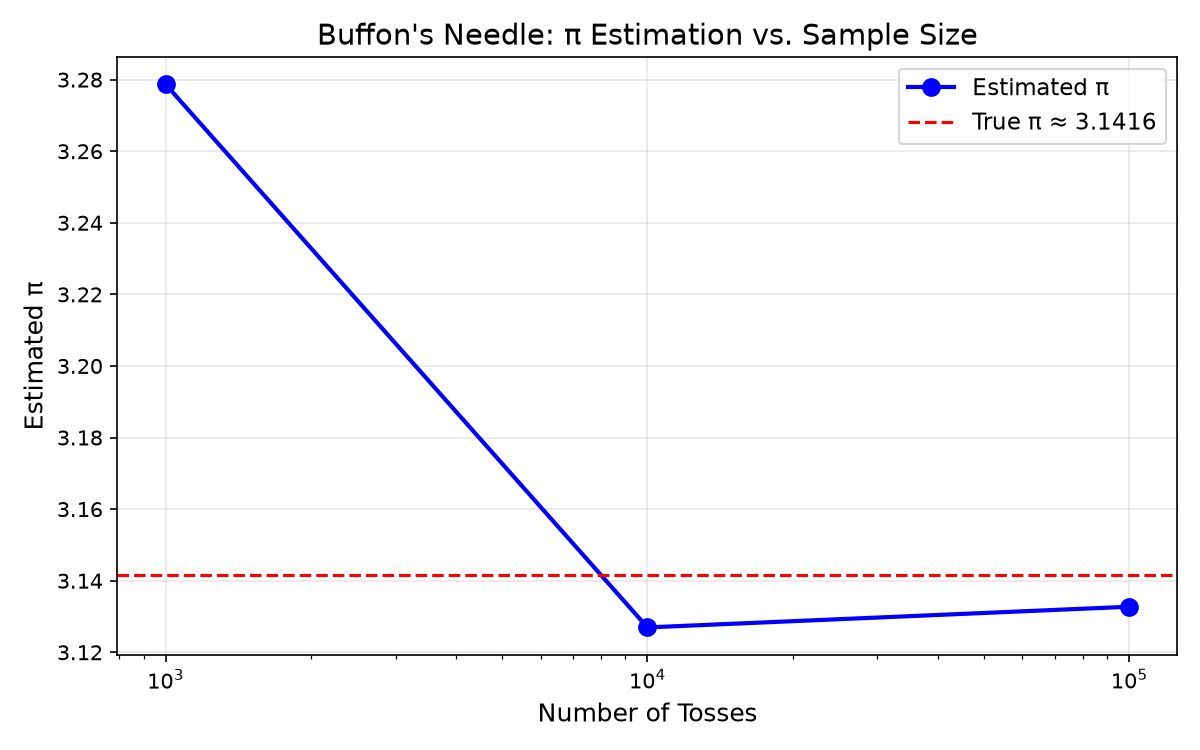
\includegraphics[width=0.8\textwidth]{results.png}
\caption{投针次数与 $\pi$ 估计值的关系}
\end{figure}

\section{结果分析}
随着投针次数的增加，$\pi$ 的估计值逐渐趋近于真实值
$\pi \approx 3.14159$。这体现了大数定律：
当试验次数足够多时，随机事件的发生频率趋近于其概率。

同时也可以看到，即使投针次数达到十万次，
估计值仍存在一定误差，这反映了随机模拟方法的统计特性。

\end{document}
